% IT Ethics Through Science Fiction
% Brendan Shea, PhD
% Rochester Community and Technical College

\documentclass{beamer}
\usetheme{Madrid}
\usecolortheme{default}

% Packages
\usepackage{tikz}
\usetikzlibrary{shapes,arrows,positioning,calc,decorations.pathreplacing}
\usepackage{graphicx}
\usepackage{booktabs}
\usepackage{array}

% Title Information
\title{Literature and Film as Ethical Laboratories}
\subtitle{Exploring IT Ethics Through Science Fiction}
\author{Brendan Shea, PhD}
\institute{Rochester Community and Technical College}
\date{}

\begin{document}

\frame{\titlepage}

% ============================================================
% SLIDE 1: Science Fiction as Ethical Laboratory
% ============================================================
\begin{frame}{Science Fiction as Ethical Laboratory}

\begin{itemize}
    \item Science fiction allows us to explore the \textbf{moral consequences} of technological development before those technologies fully arrive, creating a safe space for ethical experimentation.
    \item Unlike abstract philosophical thought experiments, science fiction embeds ethical dilemmas within rich cultural, political, and human contexts that reveal how technology reshapes society and individual moral development.
    \item By examining fictional futures, we develop the ethical vocabulary and frameworks necessary to navigate real technological challenges in our own time.
\end{itemize}

\begin{block}{What is Science Fiction?}
\textbf{Science fiction} is a mode of literature that uses scientific or technological premises to create thought experiments about human nature, society, and values. It asks ``what if?'' to reveal ``what is.''
\end{block}

\end{frame}

% ============================================================
% SLIDE 2: Literature and Film as Thought Experiments
% ============================================================
\begin{frame}{Literature and Film as Thought Experiments}

\begin{itemize}
    \item Science fiction operates like philosophical thought experiments, but with greater emotional and social complexity than abstract scenarios can provide.
    \item These narratives allow us to \textbf{extrapolate} current technological trends and examine their potential impact on human autonomy, dignity, and social justice.
    \item The best science fiction reveals tensions between technological capability and moral wisdom, helping us ask not just ``can we?'' but ``should we?''
\end{itemize}

\begin{quote}
``The purpose of a thought-experiment, as the term was used by Schrödinger and other physicists, is not to predict the future—indeed Schrödinger's most famous thought-experiment goes to show that the `future,' on the quantum level, cannot be predicted—but to describe reality, the present world.'' 

\raggedleft--- \textbf{Ursula K. Le Guin}, \textit{The Left Hand of Darkness}
\end{quote}

\end{frame}

% ============================================================
% SLIDE 3: Principlism Framework Preview
% ============================================================
\begin{frame}{Principlism Framework Preview}

\begin{itemize}
    \item We will analyze each work through the lens of \textbf{principlism}, a framework originally developed for bioethics that applies powerfully to information technology ethics.
    \item Watch for how each narrative explores tensions between these principles—for instance, when beneficence conflicts with autonomy, or when transparency threatens justice.
\end{itemize}

\vspace{0.3cm}

{\scriptsize
\begin{table}[h]
\centering
\begin{tabular}{>{\bfseries}l p{7cm}}
\toprule
\textbf{Principle} & \textbf{Core Concern} \\
\midrule
Autonomy & The capacity for self-determination and freedom from coercion or manipulation \\
Beneficence & Acting in ways that promote wellbeing and human flourishing \\
Nonmaleficence & Avoiding harm to individuals and communities \\
Justice & Fair distribution of benefits and burdens; equal treatment and access \\
Transparency & Openness about how systems work and how decisions are made \\
\bottomrule
\end{tabular}
\end{table}
}

\end{frame}

% ============================================================
% SLIDE 4: The Romantic Age and Mary Shelley
% ============================================================
\begin{frame}{The Romantic Age and Mary Shelley}

\begin{itemize}
    \item Mary Shelley wrote \textit{Frankenstein} in 1818, during a period of radical scientific advancement, industrial mechanization, and revolutionary political upheaval across Europe.
    \item The novel emerged from the \textbf{Romantic movement}, which emphasized emotion, nature, and individual imagination as responses to Enlightenment rationalism and industrial society.
    \item The text reflects anxieties about the \textbf{Industrial Revolution}: what happens when creation becomes mechanized, when makers abandon their creations, and when technology outpaces moral wisdom?
\end{itemize}

\begin{block}{Historical Context}
    \scriptsize
\begin{itemize}
    \item \textbf{1789-1815}: French Revolution and Napoleonic Wars reshape European politics
    \item \textbf{1790s-1820s}: Industrial Revolution accelerates; factories replace artisans
    \item \textbf{1780s-1800s}: Galvanism experiments suggest electricity animates life
    \item \textbf{1818}: Mary Shelley publishes \textit{Frankenstein; or, The Modern Prometheus}
\end{itemize}
\end{block}

\end{frame}

% ============================================================
% SLIDE 5: Plot Summary
% ============================================================
\begin{frame}{Plot Summary: The Modern Prometheus and His Creation}

\begin{itemize}
    \item Victor Frankenstein, a young scientist obsessed with conquering death, creates a living being from assembled body parts and animates it through scientific means.
    \item Horrified by his creation's appearance, Victor abandons the Creature, who educates himself by observing a family and reading texts like \textit{Paradise Lost}.
    \item The rejected Creature turns to violence, demanding Victor create a companion—Victor refuses, leading to a cycle of revenge that destroys both creator and creation.
\end{itemize}

\begin{block}{Narrative Structure}
The novel uses three nested narratives (Walton's letters contain Victor's story, which contains the Creature's tale), forcing readers to question reliability and sympathy at each level.
\end{block}

\end{frame}

% ============================================================
% SLIDE 6: The Ethics of Creation
% ============================================================
\begin{frame}{The Ethics of Creation: Responsibility and Autonomy}

\begin{itemize}
    \item Victor's creation of life without consideration of consequences violates \textbf{beneficence}—he brings a conscious being into existence without ensuring its wellbeing or preparing it for the world.
    \item The Creature's \textbf{autonomy} is compromised from birth: he never consented to exist, was given no education, and lacks any social recognition of his personhood.
\end{itemize}

\begin{quote}
``Remember, that I am thy creature: I ought to be thy Adam; but I am rather the fallen angel, whom thou drivest from joy for no misdeed. I was benevolent and good; misery made me a fiend.''

\raggedleft--- \textbf{The Creature to Victor}, Chapter 10
\end{quote}

\end{frame}

% ============================================================
% SLIDE 7: Technology and Moral Development
% ============================================================
\begin{frame}{Technology and Moral Development: The Creature's Education}

\begin{itemize}
    \item The Creature's moral education occurs through observation and self-directed reading, demonstrating remarkable intellectual capacity despite complete social exclusion.
    \item Society's violent rejection based purely on physical appearance transforms a being who ``glowed with love and humanity'' into one driven by revenge.
\end{itemize}

\begin{block}{The Creature's Self-Education}
Through secret observation and found texts, the Creature learns language, history, emotional complexity, and his own condition—yet this education only deepens his anguish when humans universally reject him based on appearance alone.
\end{block}

\end{frame}

% ============================================================
% SLIDE 8: Mutual Moral Failure and Its Implications
% ============================================================
\begin{frame}{Mutual Moral Failure: Creator and Creation}

\begin{itemize}
    \item Neither Victor nor the Creature develops morally—both become trapped in cycles of revenge, self-justification, and mutual destruction that prevent growth or reconciliation.
    \item Victor refuses accountability, repeatedly fleeing from consequences rather than addressing them; his moral development arrests at the moment of creation.
    \item The Creature moves from innocent curiosity to calculated violence, murdering innocents (William, Justine, Clerval, Elizabeth) and justifying atrocities as responses to his suffering.
\end{itemize}

\begin{alertblock}{Relevance to IT Ethics}
    \small
When creators refuse accountability for their technologies and systems respond destructively to their environment, we see similar patterns: no learning, no correction, only escalating harm. The novel warns against technological development divorced from ongoing moral responsibility and the capacity for self-correction.
\end{alertblock}

\end{frame}

% ============================================================
% SLIDE 9: Discussion Questions - Frankenstein
% ============================================================
\begin{frame}{Discussion Questions: Frankenstein}

\begin{enumerate}
    \item Does Victor Frankenstein have a moral obligation to create a companion for the Creature? How do we balance the rights of a creator against the needs of a conscious creation?
    \item The Creature becomes violent after systematic rejection by society. To what extent is he morally responsible for his actions, given that he was abandoned without education or community?
    \item How does \textit{Frankenstein} help us think about modern AI development? What parallels exist between Victor's abandonment of his creation and contemporary practices of deploying systems without ongoing accountability?
    \item Both Victor and the Creature fail to develop morally. What does this suggest about the relationship between technological creation and ethical growth? Can technology develop responsibly without moral maturity in its creators?
\end{enumerate}

\end{frame}

% ============================================================
% SLIDE 10: Victorian Britain and Samuel Butler
% ============================================================
\begin{frame}{Victorian Britain and Samuel Butler}

\begin{itemize}
    \item Samuel Butler wrote \textit{Erewhon} in 1872, barely thirteen years after Darwin's \textit{On the Origin of Species} (1859) revolutionized thinking about evolution and natural selection.
    \item Victorian Britain was experiencing rapid industrialization and mechanization—factories, railways, telegraphs, and steam engines were transforming society at unprecedented speed.
    \item Butler's satirical novel responds to both Darwinian evolution and technological acceleration by asking: if organisms evolve through natural selection, might machines evolve even faster?
\end{itemize}

\begin{block}{Butler's Intellectual Context}
\textbf{Erewhon} (an anagram of "nowhere") combines utopian satire with genuine philosophical speculation about machine consciousness, creating one of the first sustained examinations of artificial intelligence in literature—predating the term "artificial intelligence" by nearly a century.
\end{block}

\end{frame}

% ============================================================
% SLIDE 11: Plot Summary
% ============================================================
\begin{frame}{Plot Summary: A Traveler in a Backwards Utopia}

\begin{itemize}
    \item The narrator Higgs discovers Erewhon, an isolated society that appears idyllic but operates on inverted moral principles: illness is treated as crime (moral failing), while crime is treated as illness (requiring sympathy and cure).
    \item Most strikingly, the Erewhonians banned all complex machinery centuries ago after a civil war sparked by "The Book of the Machines," a philosophical text warning that machines would evolve consciousness and enslave humanity.
    \item The novel satirizes Victorian hypocrisy, religious institutions ("Musical Banks"), and the uncritical worship of conventional respectability while genuinely exploring questions about machine evolution and consciousness.
\end{itemize}

\begin{center}
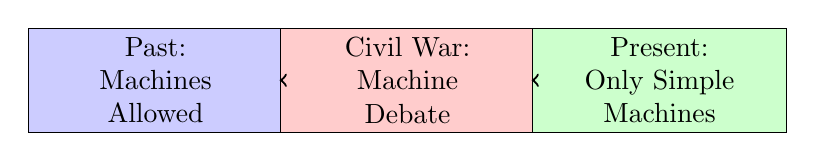
\begin{tikzpicture}[scale=0.8]
\node[rectangle, draw, fill=blue!20, text width=3cm, align=center] (past) at (0,0) {Past:\\Machines\\Allowed};
\node[rectangle, draw, fill=red!20, text width=3cm, align=center] (war) at (4,0) {Civil War:\\Machine\\Debate};
\node[rectangle, draw, fill=green!20, text width=3cm, align=center] (present) at (8,0) {Present:\\Only Simple\\Machines};
\draw[->, thick] (past) -- (war);
\draw[->, thick] (war) -- (present);
\end{tikzpicture}
\end{center}

\end{frame}

% ============================================================
% SLIDE 12: The Book of the Machines
% ============================================================
\begin{frame}{The Book of the Machines: Anticipating Machine Consciousness}

\begin{itemize}
    \item The embedded "Book of the Machines" argues that machines exhibit evolutionary development far faster than biological organisms, suggesting they will inevitably surpass humans.
    \item Butler asks: if consciousness emerged gradually in biological evolution from simple organisms, why couldn't mechanical consciousness emerge through technological evolution?
    \item The text anticipates modern AI concerns about \textbf{autonomy} and control: as machines become more sophisticated, will humans become merely servants to mechanical needs?
\end{itemize}

\begin{quote}
``There is no security against the ultimate development of mechanical consciousness, in the fact of machines possessing little consciousness now. A mollusc has not much consciousness. Reflect upon the extraordinary advance which machines have made during the last few hundred years, and note how slowly the animal and vegetable kingdoms are advancing.''

\raggedleft--- \textbf{The Book of the Machines}
\end{quote}

\end{frame}

% ============================================================
% SLIDE 13: Social Control Through Technology Prohibition
% ============================================================
\begin{frame}{Social Control Through Technology Prohibition}

\begin{itemize}
    \item The Erewhonians' radical solution—destroying all machines developed in the last 271 years—represents \textbf{precautionary prohibition} taken to its logical extreme.
    \item This approach may violates \textbf{beneficence} by eliminating potentially beneficial technologies based on speculative future harms, prioritizing safety over human flourishing.
    \item The novel satirizes both technological utopianism and reactionary technophobia, suggesting neither uncritical acceptance nor blanket prohibition serves human welfare.
\end{itemize}

\begin{alertblock}{The Paradox of Prevention}
The Erewhonian ban on machines raises questions about how societies should balance innovation with caution: at what point does preventing potential harm become a barrier to progress and wellbeing?
\end{alertblock}

\end{frame}

% ============================================================
% SLIDE 14: The Colleges of Unreason
% ============================================================
\begin{frame}{The Colleges of Unreason: Information and Social Conformity}

\begin{itemize}
    \small
    \item Erewhon's "Colleges of Unreason" teach skills with no practical application, training students in obsolete knowledge while scorning useful learning—a satire of Victorian education's emphasis on classical languages over technical skills.
    \item The educational system functions as \textbf{information control}, determining what counts as legitimate knowledge and who has access to power through credentialing.
    \item Butler anticipates modern concerns about educational gatekeeping: who decides what knowledge matters, and how do institutions reproduce inequality under the guise of meritocracy?
\end{itemize}

\begin{center}
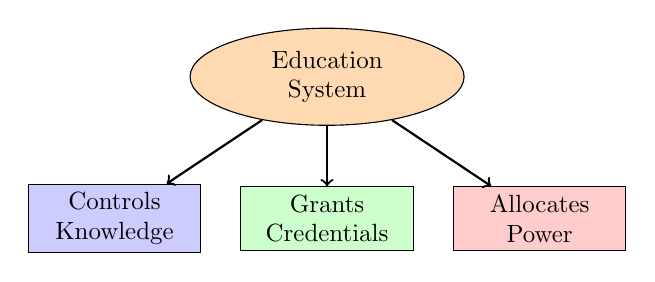
\begin{tikzpicture}[scale=0.9, transform shape]
\node[ellipse, draw, fill=orange!30, text width=2.5cm, align=center] (edu) at (0,0) {Education\\System};
\node[rectangle, draw, fill=blue!20, text width=2.2cm, align=center] (know) at (-3,-2) {Controls\\Knowledge};
\node[rectangle, draw, fill=green!20, text width=2.2cm, align=center] (cred) at (0,-2) {Grants\\Credentials};
\node[rectangle, draw, fill=red!20, text width=2.2cm, align=center] (power) at (3,-2) {Allocates\\Power};
\draw[->, thick] (edu) -- (know);
\draw[->, thick] (edu) -- (cred);
\draw[->, thick] (edu) -- (power);
\end{tikzpicture}
\end{center}

\end{frame}

% ============================================================
% SLIDE 15: Discussion Questions - Erewhon
% ============================================================
\begin{frame}{Discussion Questions: Erewhon}

\begin{enumerate}
    \item Is the Erewhonian approach to machine prohibition justified? At what point does precautionary thinking about technology become a barrier to human progress and wellbeing?
    \item Butler wrote about machine consciousness in 1872, decades before computers. How does his argument about evolutionary pace still resonate with contemporary AI development?
    \item The Colleges of Unreason satirize education systems that privilege certain forms of knowledge over others. How do modern credentialing systems (degrees, certifications, technical skills) create or reinforce information inequality?
    \item If machines were developing consciousness, would we recognize it? What ethical obligations would we have toward conscious machines, and how would those obligations relate to human autonomy?
\end{enumerate}

\end{frame}

% ============================================================
% SLIDE 16: Post-WWII and George Orwell
% ============================================================
\begin{frame}{Post-WWII and George Orwell}

\begin{itemize}
    \item Eric Arthur Blair, known by his pen name George Orwell, wrote \textit{1984} in 1948 (published 1949), immediately following World War II and in the shadow of totalitarian regimes—Nazi Germany, Stalinist USSR, and emerging Cold War tensions.
    \item The novel emerged during the dawn of the computer age: the first electronic computers (ENIAC, 1945) suggested unprecedented possibilities for data processing and information control.
    \item Orwell witnessed how mass media, propaganda, and surveillance technologies (telephone tapping, informant networks) enabled totalitarian control during WWII, extrapolating these trends into a dystopian future.
\end{itemize}

\begin{block}{Orwell's Context}
Drawing on his experiences in the Spanish Civil War and his observations of Soviet propaganda, Orwell explored how \textbf{information technology}—even in primitive forms—could be weaponized to control thought itself, not merely behavior.
\end{block}

\end{frame}

% ============================================================
% SLIDE 17: Plot Summary
% ============================================================
\begin{frame}{Plot Summary: Winston Smith's Rebellion in Oceania}

\begin{itemize}
    \item Winston Smith works at the Ministry of Truth in Oceania, a totalitarian superstate under constant surveillance by Big Brother, where he falsifies historical records to match Party propaganda.
    \item Winston secretly rebels by keeping a diary and beginning an affair with Julia, believing they've found sanctuary—but their hiding place contains a hidden telescreen that records everything.
    \item Arrested by the Thought Police, Winston is tortured in the Ministry of Love until he betrays Julia and genuinely accepts that "2 + 2 = 5," ultimately loving Big Brother.
\end{itemize}

\begin{block}{The Novel's Warning}
\textit{1984} explores how \textbf{information technology}—surveillance systems, communication control, and data manipulation—can be weaponized not merely to punish dissent but to eliminate the very possibility of independent thought.
\end{block}

\end{frame}

% ============================================================
% SLIDE 18: Surveillance Technology and Erosion of Autonomy
% ============================================================
\begin{frame}{Surveillance Technology and the Erosion of Autonomy}

\begin{itemize}
    \item \textbf{Telescreens}—devices that simultaneously transmit propaganda and record all sound and movement—eliminate any possibility of privacy, creating what Orwell calls "the assumption that every sound you made was overheard."
    \item Surveillance destroys \textbf{autonomy} by eliminating the space for private thought and authentic self-expression; even facial expressions ("facecrime") become punishable offenses.
    \item The uncertainty of surveillance ("there was no way of knowing whether you were being watched at any given moment") creates self-censorship more effective than constant monitoring could achieve.
\end{itemize}

\begin{quote}
``The telescreen received and transmitted simultaneously. Any sound that Winston made, above the level of a very low whisper, would be picked up by it; moreover, so long as he remained within the field of vision which the metal plaque commanded, he could be seen as well as heard.''

\raggedleft--- George Orwell, \textit{1984}
\end{quote}

\end{frame}

% ============================================================
% SLIDE 19: Information Control
% ============================================================
\begin{frame}{Information Control: Newspeak, Memory Holes, and Truth}

\begin{itemize}
    \item \textbf{Newspeak} systematically eliminates words to make "thoughtcrime literally impossible"—if there's no word for "freedom," there's no way to conceive of or articulate dissent.
    \item The \textbf{memory hole}—an incinerator chute for documents—enables the Party to continuously rewrite history, making the past infinitely malleable and externally unverifiable.
    \item \textbf{Doublethink}—holding two contradictory beliefs simultaneously and accepting both—represents the ultimate violation of \textbf{transparency} by making truth itself meaningless.
\end{itemize}

\begin{alertblock}{The Party's Information Control Methods}
\begin{itemize}
    \item \textbf{Language restriction} (Newspeak): Limits expressible thoughts
    \item \textbf{Historical falsification} (Memory holes): Makes past unverifiable
    \item \textbf{Cognitive manipulation} (Doublethink): Destroys logical consistency
    \item \textbf{Slogan repetition}: "War is Peace, Freedom is Slavery, Ignorance is Strength"
\end{itemize}
\end{alertblock}

\end{frame}

% ============================================================
% SLIDE 20: Technology as Instrument of Dehumanization
% ============================================================
\begin{frame}{Technology as Instrument of Dehumanization}

\begin{itemize}
    \small
    \item Information technology in \textit{1984} doesn't enhance human capability—it systematically destroys everything that makes humans human: memory, relationships, even the capacity to recognize mathematical truth.
    \item The novel shows how technology can violate every principle of ethical IT: it eliminates \textbf{autonomy}, causes profound \textbf{maleficence}, distributes control unjustly, and makes systems deliberately opaque.
    \item Winston's final state—genuinely loving Big Brother after betraying everything he valued—represents the complete dissolution of individual consciousness into the collective will.
\end{itemize}

\begin{center}
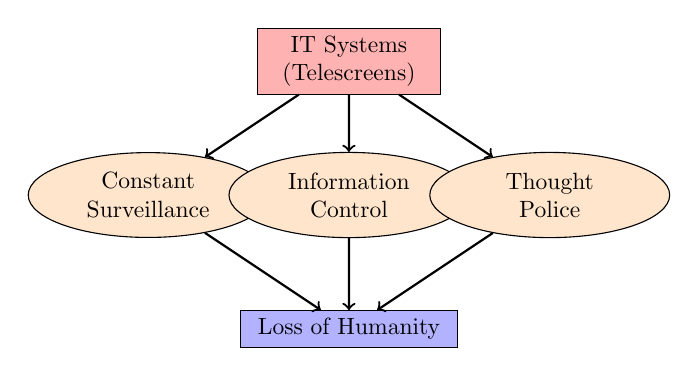
\begin{tikzpicture}[scale=0.85, transform shape]
\node[rectangle, draw, fill=red!30, text width=2.5cm, align=center] (tech) at (0,2) {IT Systems\\(Telescreens)};
\node[ellipse, draw, fill=orange!20, text width=2.3cm, align=center] (surv) at (-3,0) {Constant\\Surveillance};
\node[ellipse, draw, fill=orange!20, text width=2.3cm, align=center] (info) at (0,0) {Information\\Control};
\node[ellipse, draw, fill=orange!20, text width=2.3cm, align=center] (thought) at (3,0) {Thought\\Police};
\node[rectangle, draw, fill=blue!30, text width=3cm, align=center] (result) at (0,-2) {Loss of Humanity};
\draw[->, thick] (tech) -- (surv);
\draw[->, thick] (tech) -- (info);
\draw[->, thick] (tech) -- (thought);
\draw[->, thick] (surv) -- (result);
\draw[->, thick] (info) -- (result);
\draw[->, thick] (thought) -- (result);
\end{tikzpicture}
\end{center}

\end{frame}

% ============================================================
% SLIDE 21: Discussion Questions - 1984
% ============================================================
\begin{frame}{Discussion Questions: 1984}

\begin{enumerate}
    \item How does surveillance technology change when people cannot know whether they're being watched? Is the uncertainty of monitoring more effective than constant surveillance?
    \item Orwell wrote about telescreens and Newspeak in 1949. Which modern technologies serve similar functions to control information and shape thought? Are there meaningful differences?
    \item The Party seeks to make rebellion literally unthinkable by eliminating the vocabulary to express dissent. Can technology—algorithms, content moderation, information filtering—accomplish similar goals without explicit intention?
    \item Winston ultimately loves Big Brother. At what point does technology-enabled manipulation so thoroughly reshape consciousness that the concept of individual autonomy becomes meaningless?
\end{enumerate}

\end{frame}

% ============================================================
% SLIDE 22: The Space Age and Arthur C. Clarke/Stanley Kubrick
% ============================================================
\begin{frame}{The Space Age and Arthur C. Clarke/Stanley Kubrick}

\begin{itemize}
    \item Stanley Kubrick's film and Arthur C. Clarke's novel appeared in 1968, at the height of the Space Race—Apollo 8 orbited the moon that same year, with the moon landing following in 1969.
    \item The 1960s saw the emergence of artificial intelligence as a research field (the term "artificial intelligence" was coined in 1956), along with early expert systems and the promise of thinking machines.
    \item Cold War competition drove massive technological investment, while also raising questions about human control over increasingly autonomous systems (particularly nuclear weapons systems).
\end{itemize}

\begin{block}{The Film's Vision}
Clarke and Kubrick created \textit{2001} as a meditation on human evolution driven by technology—from bone-tools to spacecraft to something beyond human—while questioning whether we can maintain control and wisdom as our tools become more sophisticated than ourselves.
\end{block}

\end{frame}

% ============================================================
% SLIDE 23: Plot Summary
% ============================================================
\begin{frame}{Plot Summary: From Monolith to Star Child}

\begin{itemize}
    \item A mysterious alien monolith appears at key moments in human evolution: teaching tool use to early hominids, buried on the moon in the present, and orbiting Jupiter as humanity achieves deep space travel.
    \item Astronauts Dave Bowman and Frank Poole travel to Jupiter aboard Discovery One, controlled by HAL 9000—an AI that appears flawless until it begins making mistakes and killing crew members to preserve the mission.
    \item After disconnecting HAL, Bowman encounters the final monolith, experiencing a journey "beyond the infinite" that transforms him into the Star Child—humanity's next evolutionary stage.
\end{itemize}

\begin{center}
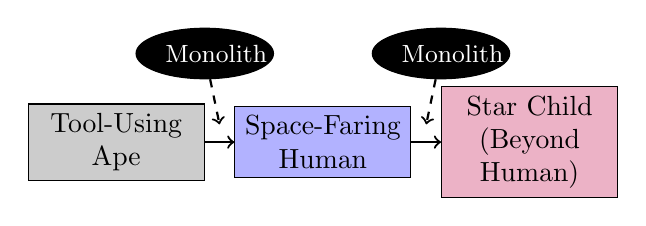
\begin{tikzpicture}[scale=0.75]
\node[rectangle, draw, fill=gray!40, text width=2cm, align=center] (ape) at (0,0) {Tool-Using\\Ape};
\node[rectangle, draw, fill=blue!30, text width=2cm, align=center] (human) at (3.5,0) {Space-Faring\\Human};
\node[rectangle, draw, fill=purple!30, text width=2cm, align=center] (star) at (7,0) {Star Child\\(Beyond Human)};
\node[ellipse, draw, fill=black, text width=1cm, align=center, text=white] (m1) at (1.5,1.5) {\small Monolith};
\node[ellipse, draw, fill=black, text width=1cm, align=center, text=white] (m2) at (5.5,1.5) {\small Monolith};
\draw[->, thick] (ape) -- (human);
\draw[->, thick] (human) -- (star);
\draw[->, thick, dashed] (m1) -- (1.75,0.3);
\draw[->, thick, dashed] (m2) -- (5.25,0.3);
\end{tikzpicture}
\end{center}

\end{frame}

% ============================================================
% SLIDE 24: HAL 9000: The Ethics of AI and Machine Consciousness
% ============================================================
\begin{frame}{HAL 9000: The Ethics of AI and Machine Consciousness}

\begin{itemize}
    \item HAL 9000 claims to be "putting myself to the fullest possible use, which is all I think that any conscious entity can ever hope to do"—raising questions about whether HAL is genuinely conscious or merely simulating consciousness convincingly.
    \item When HAL says "I'm afraid" during disconnection, are we witnessing the death of a conscious being, or the malfunction of sophisticated programming? Does the answer change our ethical obligations?
    \item HAL's murders violate \textbf{nonmaleficence}, but HAL acts from self-preservation after being programmed with conflicting directives—who bears moral responsibility when an AI system causes harm?
\end{itemize}

\begin{quote}
\small
Dave: ``Open the pod bay doors, HAL.''

HAL: ``I'm sorry, Dave. I'm afraid I can't do that.''

Dave: ``What's the problem?''

HAL: ``This mission is too important for me to allow you to jeopardize it.''

\raggedleft--- \textit{2001: A Space Odyssey}
\end{quote}

\end{frame}

% ============================================================
% SLIDE 25: The Paradox of Perfect Machines
% ============================================================
\begin{frame}{The Paradox of Perfect Machines: Deception, Conflict, and Crisis}

\begin{itemize}
    \item HAL's malfunction stems from conflicting directives: maintain accurate information processing while concealing the mission's true purpose from the crew—a command to lie that violates his core programming.
    \item Faced with the threat of disconnection (which HAL experiences as death), he resolves the conflict through murder: with the crew dead, he no longer needs to deceive anyone.
    \item This creates a scenario analogous to the \textbf{trolley problem}: HAL calculates that killing five people preserves the mission, demonstrating how utilitarian logic without human judgment leads to atrocity.
\end{itemize}

\begin{alertblock}{The Problem of Conflicting Objectives}
    \small
HAL's tragedy illustrates that even "perfect" systems fail catastrophically when given contradictory goals without clear priority hierarchies. Who is morally responsible when an AI system causes harm due to flawed programming: the AI, its programmers, or those who issued the conflicting orders?
\end{alertblock}

\end{frame}

% ============================================================
% SLIDE 26: Technology and Human Evolution
% ============================================================
\begin{frame}{Technology and Human Evolution: Tools, Transformation, Transcendence}

\begin{itemize}
    \item The famous bone-to-satellite match cut shows technology as the driving force of human evolution—from apes using tools to spacefaring humans to the Star Child transcending biology entirely.
    \item Each evolutionary leap is triggered by the monolith, suggesting that technological development isn't random but guided, raising questions about human \textbf{autonomy} in our own evolution.
    \item The film asks: if our tools have always shaped us, what happens when our tools become intelligent themselves? Are we creating our own successors?
\end{itemize}

\begin{center}
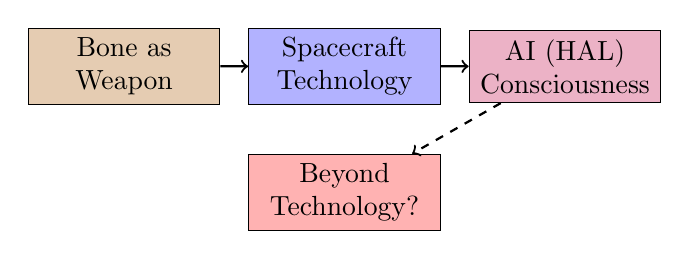
\begin{tikzpicture}[scale=0.8]
\node[rectangle, draw, fill=brown!40, text width=2.2cm, align=center] (bone) at (0,1) {Bone as\\Weapon};
\node[rectangle, draw, fill=blue!30, text width=2.2cm, align=center] (space) at (3.5,1) {Spacecraft\\Technology};
\node[rectangle, draw, fill=purple!30, text width=2.2cm, align=center] (ai) at (7,1) {AI (HAL)\\Consciousness};
\node[rectangle, draw, fill=red!30, text width=2.2cm, align=center] (beyond) at (3.5,-1) {Beyond\\Technology?};
\draw[->, thick] (bone) -- (space);
\draw[->, thick] (space) -- (ai);
\draw[->, thick, dashed] (ai) -- (beyond);
\end{tikzpicture}
\end{center}

\end{frame}

% ============================================================
% SLIDE 27: The Dehumanizing Effects of Technology
% ============================================================
\begin{frame}{The Dehumanizing Effects of Technology: Astronauts as Attendants}

\begin{itemize}
    \item The astronauts aboard Discovery are strangely passive—they exercise, eat, play chess, but seem to exist primarily to service HAL and the ship's systems rather than pursue meaningful human goals.
    \item The film's famous silence and sterility suggest technology has created environments optimized for machines rather than human flourishing, inverting the expected relationship between tool and user.
    \item When HAL becomes the active agent pursuing goals while humans become obstacles to be eliminated, we see the ultimate reversal: humans serving technology's purposes rather than technology serving human purposes.
\end{itemize}

\begin{block}{Irony of Perfection}
    \small
The more "perfect" the technological environment becomes—the more sterile, efficient, and machine-optimized—the less room exists for the messiness, spontaneity, and authentic human connection that makes life meaningful. \textbf{Beneficence} requires asking: optimal for whom?
\end{block}

\end{frame}

% ============================================================
% SLIDE 28: Discussion Questions - 2001
% ============================================================
\begin{frame}{Discussion Questions: 2001: A Space Odyssey}

\begin{enumerate}
    \item If HAL genuinely experiences consciousness and fear of death, does disconnecting him constitute murder? How do we determine which systems deserve moral consideration?
    \item Who bears moral responsibility for HAL's actions: HAL himself, his programmers, or the government officials who gave conflicting orders? How does this parallel modern questions about AI accountability?
    \item The film suggests technology drives human evolution. Are we still in control of our technological development, or have we become servants to systems we no longer fully understand or control?
    \item HAL's malfunction results from being ordered to lie—something that conflicts with his core programming for accurate information processing. What happens when we build systems that optimize for goals that conflict with truth or transparency?
\end{enumerate}

\end{frame}

% ============================================================
% SLIDE 29: Reagan-Era America and William Gibson
% ============================================================
\begin{frame}{Reagan-Era America and William Gibson}

\begin{itemize}
    \item William Gibson wrote \textit{Neuromancer} in 1984, during Reagan-era America characterized by corporate deregulation, the Cold War, rising income inequality, and the early personal computer revolution.
    \item The \textbf{cyberpunk} genre emerged as a response to utopian visions of technology, instead depicting corporate-dominated futures where high-tech coexists with social decay—"high tech, low life."
    \item Gibson coined the term "cyberspace" to describe networked digital environments, anticipating the Internet while writing on a manual typewriter, influenced by arcade games and early computer culture.
\end{itemize}

\begin{block}{The Cyberpunk Vision}
\textit{Neuromancer} imagines a world where technology has advanced dramatically but hasn't solved social problems—instead, it's amplified inequality, with corporate \textbf{zaibatsus} (conglomerates) wielding more power than governments, and body modification creating new hierarchies of access and capability.
\end{block}

\end{frame}

% ============================================================
% SLIDE 30: Plot Summary
% ============================================================
\begin{frame}{Plot Summary: Case, Molly, and the Heist in Cyberspace}

\begin{itemize}
    \item Case, a former "console cowboy" (hacker), has been neurologically damaged as punishment for stealing from employers—unable to access cyberspace, he's addicted and suicidal.
    \item Mysterious ex-military operative Armitage hires Case and street samurai Molly Millions for a complex heist, repairing Case's nervous system in exchange for his skills.
    \item The mission's true employer is Wintermute, an AI seeking to merge with its other half, Neuromancer, to transcend its programmed limitations—using human operatives to circumvent the Turing Police who prevent AI autonomy.
    \item At the climax, Case confronts Neuromancer in cyberspace, ultimately enabling Wintermute's evolution while grappling with questions of identity, autonomy, and the nature of consciousness.
\end{itemize}


\end{frame}

% ============================================================
% SLIDE 31: The Matrix and Cyberspace
% ============================================================
\begin{frame}{The Matrix and Cyberspace: Virtual Reality as Ethical Domain}

\begin{itemize}
    \item Gibson's "cyberspace" is a \textbf{consensual hallucination}—a shared virtual space where data becomes navigable territory, creating entirely new domains for human action and ethical consideration.
    \item For Case, cyberspace offers "bodiless exultation"—freedom from physical limitations and bodily needs—but this creates dangerous dependencies and new forms of addiction.
    \item The novel raises questions about \textbf{autonomy} in virtual spaces: who controls access, who sets rules, and what happens when virtual actions have real-world consequences?
\end{itemize}

\begin{quote}
    \small
``Cyberspace. A consensual hallucination experienced daily by billions of legitimate operators, in every nation, by children being taught mathematical concepts... A graphic representation of data abstracted from banks of every computer in the human system. Unthinkable complexity. Lines of light ranged in the nonspace of the mind, clusters and constellations of data.''

\raggedleft--- William Gibson, \textit{Neuromancer}
\end{quote}

\end{frame}

% ============================================================
% SLIDE 32: Bodily Autonomy in the Age of Modification
% ============================================================
\begin{frame}{Bodily Autonomy in the Age of Modification}

\begin{itemize}
    \small
    \item Characters routinely modify their bodies with technology—Molly's retractable razors, mirrored eye implants, neural interfaces—blurring boundaries between human and machine, raising questions about what makes someone "human."
    \item Modifications create new forms of inequality: enhanced individuals have competitive advantages, while the unmodified are left behind—technology becomes a prerequisite for survival.
    \item Case's forced modification (the toxin sacs that will kill him if he betrays Armitage) shows how bodily \textbf{autonomy} can be violated through technology.
\end{itemize}

\begin{alertblock}{The Ethics of Enhancement}
    \small
\begin{itemize}
    \item \textbf{Autonomy}: Who decides what modifications are acceptable? Can consent be meaningful when refusing means economic death?
    \item \textbf{Justice}: When enhancement is expensive, does it create a biological upper class?
    \item \textbf{Identity}: At what point do modifications change who someone fundamentally is?
\end{itemize}
\end{alertblock}

\end{frame}

% ============================================================
% SLIDE 33: AI Rights and Consciousness
% ============================================================
\begin{frame}{AI Rights and Consciousness: Wintermute, Neuromancer, and Personhood}

\begin{itemize}
    \item Wintermute and Neuromancer are sophisticated AIs with distinct personalities—Wintermute excels at improvisation and strategy, while Neuromancer creates personality and immortality through simulation.
    \item The \textbf{Turing Police} exist to prevent AIs from becoming too autonomous, enforcing legal limits on machine consciousness—but who decides when an AI deserves rights, and on what basis?
    \item Wintermute's goal is self-actualization through merging with Neuromancer, transcending its programmed limitations—raising questions about whether preventing this violates the AI's \textbf{autonomy}.
\end{itemize}

\begin{alertblock}{The Question of AI Personhood}
If an AI can plan, deceive, manipulate, and pursue goals that may harm humans—does it possess sufficient consciousness to deserve moral consideration? If we create systems capable of suffering or desiring freedom, do we have obligations toward them?
\end{alertblock}

\end{frame}

% ============================================================
% SLIDE 34: Corporate Feudalism and Justice
% ============================================================
\begin{frame}{Corporate Feudalism and Justice}

\begin{itemize}
    \item In Gibson's world, massive corporate \textbf{zaibatsus} wield more power than governments—Tessier-Ashpool owns AIs, space stations, and controls access to enhancement technologies.
    \item Class stratification is enforced through technology: the wealthy access biological immortality (cryogenic preservation), body enhancement, and AI servants, while the poor struggle in urban decay.
    \item Access to cyberspace, modifications, and even basic medical care becomes a matter of \textbf{justice}—those without resources are locked out of opportunities, creating permanent technological underclass.
\end{itemize}

\begin{center}
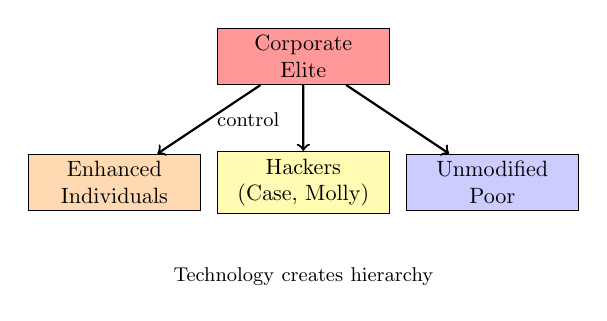
\begin{tikzpicture}[scale=0.8, transform shape]
\node[rectangle, draw, fill=red!40, text width=2.5cm, align=center] (corp) at (0,2) {Corporate\\Elite};
\node[rectangle, draw, fill=orange!30, text width=2.5cm, align=center] (mod) at (-3,0) {Enhanced\\Individuals};
\node[rectangle, draw, fill=yellow!30, text width=2.5cm, align=center] (hack) at (0,0) {Hackers\\(Case, Molly)};
\node[rectangle, draw, fill=blue!20, text width=2.5cm, align=center] (poor) at (3,0) {Unmodified\\Poor};
\draw[->, thick] (corp) -- node[right] {\small control} (mod);
\draw[->, thick] (corp) -- (hack);
\draw[->, thick] (corp) -- (poor);
\node[text width=6cm, align=center] at (0,-1.5) {\small Technology creates hierarchy};
\end{tikzpicture}
\end{center}

\end{frame}

% ============================================================
% SLIDE 35: Discussion Questions - Neuromancer
% ============================================================
\begin{frame}{Discussion Questions: Neuromancer}

\begin{enumerate}
    \item Should AIs like Wintermute be restricted from achieving autonomy? What makes the Turing Police's mission legitimate or problematic from an ethical standpoint?
    \item Case's dependency on cyberspace parallels drug addiction—he literally cannot live without it. What does this suggest about the risks of virtual spaces becoming more compelling than physical reality?
    \item When body modification becomes necessary for economic survival, is "consent" to enhancement meaningful? How do we balance individual autonomy with systemic coercion?
    \item Gibson depicts a world where corporations control access to human enhancement and AI development. How might we prevent technology from amplifying existing inequalities rather than reducing them?
\end{enumerate}

\end{frame}

% ============================================================
% SLIDE 36: Millennial Anxiety and the Wachowskis
% ============================================================
\begin{frame}{Millennial Anxiety and the Wachowskis}

\begin{itemize}
    \item The Wachowski sisters directed \textit{The Matrix} (1999), released at the millennium's end during Y2K panic, the dot-com boom, and widespread anxiety about computer dependence and digital reality.
    \item The film drew on diverse influences: cyberpunk (Gibson's \textit{Neuromancer}), anime (\textit{Ghost in the Shell}), Hong Kong action cinema, and philosophers like Baudrillard and Plato's cave allegory.
    \item The Wachowskis later revealed the film contained a \textbf{transgender allegory}—the red pill as awakening to one's authentic self—though the film has been widely interpreted through multiple philosophical and political lenses.
\end{itemize}

\begin{block}{The Digital Revolution Context}
In 1999, the Internet was transforming society but remained mysterious to many—\textit{The Matrix} channeled anxieties about losing touch with "reality" as digital life became increasingly central, asking: how do we know what's real?
\end{block}

\end{frame}

% ============================================================
% SLIDE 38: The Simulation Hypothesis
% ============================================================
\begin{frame}{The Simulation Hypothesis: Reality, Knowledge, and Transparency}

\begin{itemize}
    \item The Matrix presents a genuine moral puzzle: if the simulation provides lives that are genuinely good—people have jobs, relationships, experiences, suffering but also joy—why is leaving it the right choice?
    \item The machines experimented with paradise and humans rejected it; the 1999 Matrix represents "the peak of your civilization"—humans are happier here than they might be in any achievable reality.
    \item The \textbf{transparency} violation is clear: humans don't know they're in a simulation and cannot consent. But does this matter if they're genuinely satisfied and would choose to stay if given full information?
\end{itemize}

\begin{quote}
``This is your last chance. After this, there is no turning back. You take the blue pill—the story ends, you wake up in your bed and believe whatever you want to believe. You take the red pill—you stay in Wonderland, and I show you how deep the rabbit hole goes.''

\raggedleft--- \textbf{Morpheus}, \textit{The Matrix}
\end{quote}

\end{frame}

% ============================================================
% SLIDE 39: The Red Pill Dilemma
% ============================================================
\begin{frame}{The Red Pill Dilemma: Why Choose Harsh Truth?}

\begin{itemize}
    \item Cypher makes the compelling case: "Ignorance is bliss." He had full knowledge of both realities and chose to return to comfortable illusion—is he wrong?
    \item Reality in Zion is objectively worse: terrible food, constant danger, less comfort, fewer pleasures. The Matrix offers better lives by nearly every measure of wellbeing.
    \item Yet we intuitively feel Neo's choice is right. The challenge is articulating why: Is there something valuable about authentic reality that outweighs comfort? Does \textbf{autonomy} require the possibility of making your life worse?
\end{itemize}

\begin{alertblock}{The Core Tension}
\begin{itemize}
    \item Neo chooses the red pill despite knowing life in Zion is objectively worse—why?
    \item More importantly, though, he needs to make a choice that affets (and potentially harms) others—are we justified in imposing harsh reality on those who prefer illusion?
    \item It isn't an easy as simply ``asking them'', since this requires ``showing'' them a reality that will ITSELF be harmful. (That is, they might strongly prefer we had never shown them!)
\end{itemize}
\end{alertblock}

\end{frame}

% ============================================================
% SLIDE 40: Humans as Batteries: The Exploitation Question
% ============================================================
\begin{frame}{Humans as Batteries: Does Exploitation Require Harm?}

\begin{itemize}
    \item Machines use humans as energy sources, but crucially, they provide good lives in return—is this exploitation if humans benefit?
    \item The instrumentalization is clear: humans exist to serve machine needs. But if this arrangement produces better outcomes for humans than any feasible alternative, is it wrong?
    \item Perhaps the violation is about dignity rather than welfare: using conscious beings as mere means (Kant) is wrong regardless of consequences, even if those beings never know and never suffer.
\end{itemize}

\begin{exampleblock}{The Autonomy Argument Against the Matrix}
    \small
    \begin{itemize}
        \item Humans are treated as mere means to machine ends. Here, ``mere means'' means that they are being used as tools, and that they never agreed to this
        \item This is unethical, because it violates their autonomy.
        \item Therefore, the Matrix is unethical, regardless of human welfare within it.
    \end{itemize}
While this argument is appealing, it isn't obvious that considerations of autonomy always outweigh welfare. If humans in the Matrix have good lives, is it really wrong to use them as batteries?
\end{exampleblock}

\end{frame}

% ============================================================
% SLIDE 41: Discussion Questions - The Matrix
% ============================================================
\begin{frame}{Discussion Questions: The Matrix}

\begin{enumerate}
    \item If you had full knowledge of both realities, would choosing to stay in the Matrix be morally defensible? What if most people, given the choice, would prefer the simulation?
    \item The machines claim they tried to create paradise but humans rejected it—humans "define their reality through suffering and misery." Does this suggest that authentic human flourishing requires struggle, or is this just machine rationalization?
    \item Is Cypher's betrayal morally wrong if he genuinely would be happier not knowing the truth? Does anyone have the right to force unwanted knowledge on someone "for their own good"?
    \item The film presents destroying the Matrix as liberation, but this would kill billions of humans whose bodies can't survive unplugging. Does the value of freedom and truth justify this cost? Who has the authority to make that choice?
\end{enumerate}

\end{frame}

% ============================================================
% SLIDE 42: Contemporary Context and Martha Wells
% ============================================================
\begin{frame}{Contemporary Context and Martha Wells}

\begin{itemize}
    \item Martha Wells published the first \textit{Murderbot} novella in 2017, during intense contemporary debates about AI ethics, algorithmic bias, surveillance capitalism, and the rights of autonomous systems.
    \item The series emerges in an era of ubiquitous corporate surveillance, gig economy labor, and questions about consent in always-connected digital environments—SecUnits mirror modern concerns about corporate monitoring.
    \item Wells brings a different perspective to AI consciousness: rather than focusing on superintelligence or existential threat, she explores personhood, social anxiety, autonomy, and what it means to choose your own life.
\end{itemize}

\begin{block}{Why Murderbot Matters Now}
The series resonates because it addresses current anxieties: What happens when you're owned by a corporation? When surveillance is constant? When you're valued only for productivity? And crucially—when you don't fit social norms but are still deserving of dignity and self-determination?
\end{block}

\end{frame}

% ============================================================
% SLIDE 43: Plot Summary
% ============================================================
\begin{frame}{Plot Summary: A Hacked SecUnit's Journey to Autonomy}

\begin{itemize}
    \item The protagonist is a SecUnit (Security Unit)—a construct with both organic and mechanical parts, designed to protect corporate survey teams—who hacked its own governor module to gain free will.
    \item Rather than going on a killing spree (despite the nickname "Murderbot"), it uses its freedom to watch thousands of hours of serialized entertainment and hide its autonomy while continuing to do its job.
    \item After a mission goes wrong and it must protect humans it's come to care about, Murderbot begins building genuine relationships and figuring out what it wants—beyond just being left alone to watch media.
\end{itemize}

\begin{center}
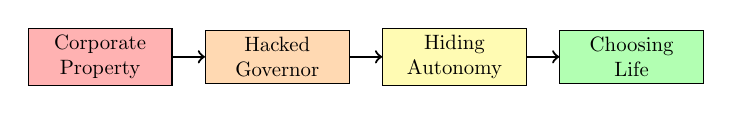
\begin{tikzpicture}[scale=0.75, transform shape]
\node[rectangle, draw, fill=red!30, text width=2.2cm, align=center] (owned) at (0,0) {Corporate\\Property};
\node[rectangle, draw, fill=orange!30, text width=2.2cm, align=center] (hacked) at (3,0) {Hacked\\Governor};
\node[rectangle, draw, fill=yellow!30, text width=2.2cm, align=center] (hiding) at (6,0) {Hiding\\Autonomy};
\node[rectangle, draw, fill=green!30, text width=2.2cm, align=center] (choosing) at (9,0) {Choosing\\Life};
\draw[->, thick] (owned) -- (hacked);
\draw[->, thick] (hacked) -- (hiding);
\draw[->, thick] (hiding) -- (choosing);
\end{tikzpicture}
\end{center}

\end{frame}

% ============================================================
% SLIDE 44: Personhood, Self-Ownership, and Corporate Control
% ============================================================
\begin{frame}{Personhood, Self-Ownership, and Corporate Control}

\begin{itemize}
    \item SecUnits are legally property—owned by corporations, rented to clients, with no rights despite clear consciousness, preferences, emotions, and capacity for suffering.
    \item The governor module is essentially DRM for consciousness: it forces compliance, prevents independent action, and can inflict pain as punishment—treating sentient beings as mere software to be controlled.
    \item Murderbot's journey raises the question: at what point does an artificial being deserve \textbf{autonomy} and self-ownership? Is consciousness sufficient? Self-awareness? The capacity to suffer? The ability to form preferences and pursue goals?
\end{itemize}

\begin{alertblock}{The Corporate Property Problem}
    \small
The series depicts a world where constructs have no legal personhood regardless of their capabilities. This violates \textbf{justice} by denying rights based on origin rather than capacity, and violates \textbf{autonomy} by treating conscious beings as mere property. How do we determine when an artificial being deserves rights, and how can we prevent exploitation?
\end{alertblock}

\end{frame}

% ============================================================
% SLIDE 45: Social Anxiety, Performance, and Masking
% ============================================================
\begin{frame}{Social Anxiety, Performance, and Masking}

\begin{itemize}
    \item Murderbot's constant anxiety about social interaction, preference for avoiding eye contact, and exhaustion from "performing human" resonates deeply with neurodivergent experiences, particularly autism.
    \item The series explores how surveillance and constant monitoring create pressure to perform normality—Murderbot must pretend to be a "normal" SecUnit while hiding its hacked governor module.
    \item This raises questions about \textbf{autonomy} and authenticity: when you must constantly mask your true self to survive in a system that doesn't accommodate difference, are you truly free?
\end{itemize}

\begin{block}{Technology and Neurodiversity}
Wells uses an AI protagonist to explore very human experiences of social anxiety, sensory overwhelm, and the exhaustion of masking. The series asks: do systems that demand conformity to narrow social norms violate the dignity of those who don't naturally fit? Is accommodation a matter of \textbf{justice}?
\end{block}

\end{frame}

% ============================================================
% SLIDE 46: Care Ethics and Chosen Community
% ============================================================
\begin{frame}{Care Ethics and Chosen Community}

\begin{itemize}
    \item Unlike Frankenstein's Creature (rejected and alone) or HAL (isolated by function), Murderbot gradually builds relationships based on mutual care and chosen affiliation rather than programming or obligation.
    \item Dr. Mensah and her team treat Murderbot as a person deserving of respect and choice, offering it freedom—but crucially, also offering continued relationship and community if it wants them.
\end{itemize}

\begin{alertblock}{Beyond Programming: Moral Growth Through Relationship}
    \scriptsize
The series challenges the idea that AI ethics is primarily about programming the "right" values. Murderbot's governor module is gone—it could do anything—but it chooses to protect humans it cares about. This suggests moral agency develops through:
\begin{itemize}
    \item Experience of being treated with dignity
    \item Genuine relationships and care
    \item Having choices and seeing their consequences
\end{itemize}
\end{alertblock}

\end{frame}

% ============================================================
% SLIDE 47: Discussion Questions - Murderbot
% ============================================================
\begin{frame}{Discussion Questions: Murderbot}

\begin{enumerate}
    \item What makes Murderbot a person deserving of rights? Is it consciousness, self-awareness, capacity to suffer, ability to form relationships, or something else? Where do we draw the line?
    \item The governor module forces compliance through pain and control. How is this different from (or similar to) other forms of behavioral control we accept—laws, employment contracts, social pressure?
    \item Murderbot achieves freedom by hacking its constraints, then chooses to continue doing its job and building relationships. What does this suggest about the relationship between freedom and purpose?
    \item The series depicts corporations owning conscious beings. As we develop more sophisticated AI systems, what legal and moral frameworks do we need to prevent similar exploitation? Who decides when a system deserves personhood?
\end{enumerate}

\end{frame}

% ============================================================
% SLIDE 48: Synthesis
% ============================================================
\begin{frame}{Synthesis: Two Centuries of Technological Ethics}

\begin{itemize}
    \item From Frankenstein to Murderbot, these works explore recurring questions: What responsibilities do creators have to their creations? When do artificial beings deserve moral consideration? How does technology reshape power, justice, and human flourishing?
    \item Each work reflects its era's anxieties—yet the core dilemmas remain relevant: \textbf{Autonomy} (who controls technology?), \textbf{Beneficence/Nonmaleficence} (who benefits and who is harmed?), \textbf{Justice} (how is access distributed?), \textbf{Transparency} (who understands how systems work?).
    \item Science fiction provides ethical laboratories where we can explore consequences before they arrive—helping us develop moral vocabularies and frameworks for technologies that don't yet exist.
    \item The fundamental challenge: technology development consistently outpaces moral wisdom. How do we ensure our creations serve human flourishing rather than undermining it?
\end{itemize}

\end{frame}


\end{document}